\documentclass[11pt,letterpaper]{article}
\usepackage{naaclhlt2015}
\usepackage{times}
\usepackage{latexsym}
\usepackage{url}
\usepackage[pdftex]{graphicx}
\setlength\titlebox{6.5cm}    % Expanding the titlebox

%%%%%%%%%%%%%%%%%%%%%%%%%%%%%%%%%%%%%%%%%%%%%%%%%%%%%%%%%%%%%%%%%%%%%%
% Code to use with NAACL/ACL style files to simulate natbib's 
% \citealt, which prints citations with no parentheses. This should
% work if pasted into the preamble. \cite, \newcite, and \shortcite
% should continue to work as before.

\makeatletter

\def\citealt{\def\citename##1{{\frenchspacing##1} }\@internalcitec}

\def\@citexc[#1]#2{\if@filesw\immediate\write\@auxout{\string\citation{#2}}\fi
  \def\@citea{}\@citealt{\@for\@citeb:=#2\do
    {\@citea\def\@citea{;\penalty\@m\ }\@ifundefined
       {b@\@citeb}{{\bf ?}\@warning
       {Citation `\@citeb' on page \thepage \space undefined}}%
{\csname b@\@citeb\endcsname}}}{#1}}

\def\@internalcitec{\@ifnextchar [{\@tempswatrue\@citexc}{\@tempswafalse\@citexc[]}}

\def\@citealt#1#2{{#1\if@tempswa, #2\fi}}

\makeatother
%%%%%%%%%%%%%%%%%%%%%%%%%%%%%%%%%%%%%%%%%%%%%%%%%%%%%%%%%%%%%%%%%%%%%%

% Effects of non-linguistic context
\title{Shared common ground influences information density in microblog texts\Thanks{Thanks to...}}
% common ground decreases information

\author{Gabriel Doyle\\
	    Stanford University\\
	    450 Serra Mall\\
	    Stanford, CA 94305, USA\\
	    {\tt gdoyle@stanford.edu}
	  \And
          Michael C. Frank\\
	    Stanford University\\
	    450 Serra Mall\\
	    Stanford, CA 94305, USA\\
	    {\tt mcfrank@stanford.edu}}

\date{}


\begin{document}
\maketitle
\begin{abstract}
Natural languages offer many possible ways to say the same thing. If speakers use language rationally, they should structure their messages to achieve approximately uniform information density (UID), maximizing tranmission via a noisy channel. One signature of UID identified by previous work is the consistent increase in linguistic information across sentences in text. Such an increase implies a corresponding increase in shared non-linguistic common ground. We test this prediction for the first time, using microblog texts from twitter. We take advantage of tweets about a single shared event---the World Series of baseball---to measure common ground, identifying both gradual and rapid changes in information content in response to in-game events. These findings lend further support to the UID hypothesis and underscore the importance of non-linguistic common ground for language understanding.
\end{abstract}

\section{Introduction}

Natural language is an incredibly powerful method for representing and communicating information. One consequence of this power is that there is an infinity of different ways to structure any particular message. How do speakers choose between different possible structures? One provocative hypothesis is that they attempt to structure their message to best convey their intended meaning, conditioned on the myriad aspects of the particular channel (whether spoken or written, noisy or not), listener (whether friend, acquaintance, or strange), and context (whether a decontextualized written statement or a comment on a joint activity, or any situation in between). 

On this view, the use of natural languages is assumed to follow many of the patterns of optimal information transmission derived via information theory \cite{shannon1948}. In particular, speakers should structure their messages to approximate \emph{uniform information density}, a feature which is optimal for transmission of information through a noisy channel. Recent research has suggested ways in which natural language samples---and by extension, the speakers generating these samples---seem to follow this regularity. In line with this prediction, speakers omit optional lexical material in cases where the subsequent syntactic information is relatively more predictable \cite{levy2007,frank2008,jaeger2010}. They also pursue phonological reduction for more predictable material \cite{aylett2004,aylett2006}. Predictability in both these examples is defined within the sentential context, however. 

Another body of evidence concerns changes in linguistic information content as shared common ground is built up. Following the UID hypothesis, \citealt{genzel2002} proposed that $H(Y_i)$, the total entropy of part $i$ of a message, is constant. They factor this expression by considering $X_i$, the random variable representing the word that will appear at position $i$, conditioned on all the previous observed words. They then further factor this expression into two terms:

\begin{eqnarray}
H(Y_i) &=& H(X_i | C_i, L_i) \\
&=& H(X_i | L_i) - I(X_i | C_i, L_i)
\end{eqnarray}

\noindent where the first term $H(X_i | L_i)$ is the dependence of the current word on the local linguistic context (e.g. within the rest of the sentence $L_i$) and the second is the mutual information between the current word and the broader linguistic context $C_i$, given the current sentence. On their logic, given greater amounts of contextual information, $I(X_i | C_i, L_i)$ must go up. Therefore, they predicted that $H(X_i|L_i)$ should also increase, so as to result in a constant total amount of information. They then approximated $H(X_i | L_i)$ using a number of methods and showed that indeed it did increase systematically in documents. Later work showed that this increase was strongest within paragraphs and was general across document types \cite{genzel2003} and languages \cite{qian2012}.

In all of this work, however, context has been defined in purely linguistic terms---likely for practical reasons, rather than theoretical ones. In psycholinguistics, the notion of shared \emph{common ground} is a more precise replacement for the general notion of ``context'' and is assumed to subsume \emph{both} linguistic and non-linguistic context \cite{stalnaker1978,clark1996}, constituting the total sum of knowledge that communicators share with their audience. A broad literature suggests that speakers consider common ground in selecting the appropriate expression to refer to a particular object \cite{brennan1996,metzing2003}. 

In principle, Genzel and Charniak's context term can be considered as capturing common ground. Although they stated the regularity in terms of mutual information between the current word and the context, an alternative formulation would be in terms of the total information content of the current word and the context. 

\begin{equation}
H(Y_i) = H(X_i | L_i) + H(C_i) = FIXME
\end{equation}

\noindent We consider the possibility that we can measure $H(C_i)$ directly via common ground. 

In the current paper we use twitter, a popular microblogging service, to operationalize common ground and assess its relationship with the information density of individual messages. Because of its structure, twitter is an ideal platform for this investigation. One common method of using twitter is to mark messages with hashtags, which makes them viewable and searchable to the entire twitter audience. This strategy is especially used when users are commenting on an external event (e.g. a sporting, media, or political event). We focus here on the World Series of baseball, an annual sporting event with large viewership; in this case, the hashtag is \texttt{\#worldseries}. Hashtagged messages thus form a case in which there is \emph{no} prior linguistic context. The total shared context with the audience that can be assumed by the writer of a tweet is the non-linguistic content of the event being hashtagged. 

We make use of this feature to investigate the possibility of a reciprocal relationship between the linguistic complexity of tweets and the amount of shared common ground related to the ongoing event. We begin by describing our corpus and our method of calculating linguistic content (by computing entropy within a simple $n$-gram model). We then investigate gradual changes in word-by-word information content as the event goes on and rapid changes in the total information content of tweets in response to important in-game events. We end by considering a number of control analyses that provide evidence against alternative accounts of our results. 

\section{Corpus and Methods}

\subsection{\#worldseries Corpus}

Our current analysis looks at tweets during the 2014 World Series, a series of seven baseball games.  We obtained these tweets using an adaptation of SeeTweet \cite{doyle2014} to search for tweets containing the hashtag ``\#WorldSeries.''  To synchronize tweets with game events, we used the Major League Baseball Advance Media XML repository,\footnote{\url{http://gd2.mlb.com/components/game/mlb/}} which contains pitch-by-pitch data including the ongoing state of the game and timestamps of events. Using timestamp information, we bin tweets by at-bats (so that they can be effectively co-registered with other in-game statistics).  We limit our analysis to tweets timestamped during the game, resulting in a total corpus of 109,207 tweets.

These tweets are compiled from the ``garden-hose'' Twitter search API, which returns a subset of all relevant tweets. In practice, our searches catch approximately 4\% of all relevant tweets; Twitter reported 420,329 relevant tweets during Game 1 of the World Series\footnote{\url{https://twitter.com/TwitterData/status/524972545930301440}}, and our dataset contained 17,538 tweets during the same time period.

\subsection{Entropy Computation}

We computed the linguistic information content of each tweet in our corpus. Social media text has been described as ``bad language'' \cite{eisenstein2013}, and can be difficult to model due to its idiosyncratic abbreviations, typographic errors, and other non-standard forms. Relevant to our goal of assessing information content, it can be difficult to create an appropriate training corpus for language models, since vocabulary and composition of tweets of change substantially on both short and long timescales \cite{eisenstein2013}.

We attempted to minimize these difficulties in two ways.  First, we used tweet length (in characters) as our initial metric of information content. Unless information rate varies systematically across tweets of different lengths---counter to the claim of approximately uniform information density in language\cite{genzel2002,levy2007}---longer tweets will generally carry more information.

Second, we estimated language models with domain-specific corpora. In particular, for tweets from each game we used a training corpus consisting of the tweets from all the other games. This training set provided a vocabulary and structure that was similar in topic and style and to the test set.  We removed all punctuation and emoji except word-initial {\it @} and {\it \#}, which refer to users and hashtags, respectively.  Usernames were replaced with {\it [MENTION]} to reduce sparsity; hashtags were not altered, as these often function as words or phrases within the tweet's syntax.  Words with fewer than 5 occurrences in the training corpus were marked as out-of-vocabulary items.

We estimated trigram models using a modification of NLTK \cite{bird2006} with Witten-Bell smoothing, and computed information content as

\begin{equation}
H_L = \sum_i{p ~ log(p)} - FIXME
\end{equation}

\section{Gradual Changes in Information Rate}

Our first analytic goal was to examine changes in the information content of tweets over the course of a shared event.  We predicted that we would see similar developments in information structure as in more traditional conversational settings, even though there was no formal conversation.  Specifically, we predicted that the build-up of contextual information would cause the context-independent per-word entropy to rise over time, replicating an effect that has been observed across languages and genres\cite{genzel2002,genzel2003,qian2012}.

\begin{figure}
 \centering
  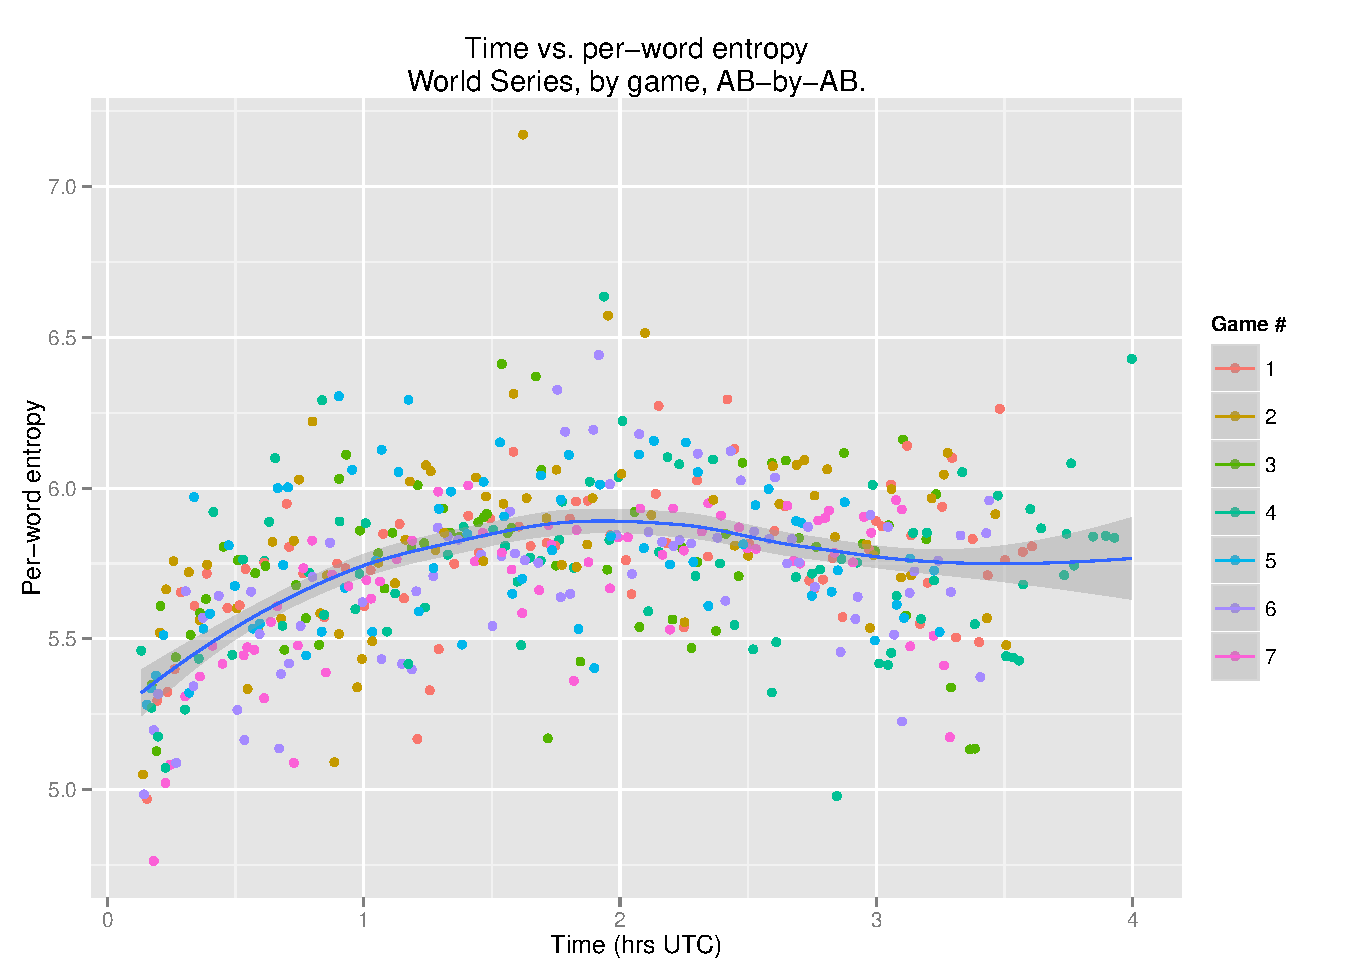
\includegraphics[width=3.25in]{figures/time-perword-ent-agg}
 \caption{Per-word entropy increases with time for the first two hours of the games, then levels off and slightly declines. Loess curve fitting with 95\% confidence intervals.}\label{fig:time-perword-ent}\vspace*{-.5em}
\end{figure}

\begin{table*}
  \begin{tabular}{clc}
 Minute & Tweet & Per-word entropy \\
\hline
0 & \#WorldSeries Play Ball & 4.96\\
0 & It's finally here! \#WorldSeries & 4.74\\
0 & \parbox[][6ex][c]{.7\textwidth}{IDEA: @mayoredlee, \#SanFrancisco can pledge to throw our @SFGiants an \#OrangeOctober parade regardless of \#WorldSeries outcome! \#SFGiants} & 8.20\\
\hline
12 & The guy with the Marlins sweater is behind home plate again. \#worldseries & 4.26\\
12 & \parbox[][6ex][c]{.7\textwidth}{Something about Hunter Pence really, really bothers me. Don't ask me what, cause I havent figured it out, but I don't like him. \#WorldSeries} & 6.64\\
12 & The Giants 3-0! \#WorldSeries & 5.43\\
\hline
73 & \parbox[][6ex][c]{.7\textwidth}{Three HORRIBLE at-bats (mixed in with Cain's walk) prevent Royals from breaking through in the third. \#WorldSeries} & 9.39\\
130 & \parbox[][6ex][c]{.7\textwidth}{As Hardy Boy \#2, Joe Panik just pulled the mask off of Vargas and discovered it's Old Man Withers from down the street. \#WorldSeries} & 8.12\\
178 & \parbox[][6ex][c]{.7\textwidth}{\#WorldSeries it's funny the non body names have a great hits. Frm now n on consider the Postseson as Cinderla run.  No names needed, \#MLB} & 10.04\\
\hline
  \end{tabular}
 \caption{Example tweets, grouped by time since first pitch.}\label{tab:ex}
\end{table*}

Figure \ref{fig:time-perword-ent} shows evidence for changes in per-word entropy over the course of games. 
Per-word entropy rises sharply in the first half-hour of each games, then begins to level off and finally declines slightly over time.  This pattern is consistent with the constant entropy rate proposal of \cite{genzel2002}, and more specifically with the context decay model of \cite{qian2012}.\footnote{A late decline in per-word entropy also appeared in \cite{qian2012}'s analysis of Swedish.}  

A later tweet with the same in-context entropy as an earlier tweet will have a higher entropy when estimated out-of-context. We hypothesize that this finding is due to the accrual of common ground across users. As they watch more of the game, they share more referents and have stronger expectations about the shape of the game. This shared common ground licenses more complex language and more sophisticated linguistic references. Table \ref{tab:ex} gives example tweets at different time points; references expand from mostly generic team/series references to specific individuals and events, and eventually to include sequences of events.

While this finding is consistent with previous work on the effect of context \cite{genzel2002,qian2012}, it expands the definition of context.  In previous work, the context came from explicit linguistic information, as it tested written paragraphs.  In the Twitter dataset, the context comes from real-world events during the games, as there is no canonical shared sequence of tweets that the tweeters can refer back to.  Contextual influences on entropy need not be explicitly linguistic.

\section{Fast Changes In Information Content}

\begin{figure}
 \centering
  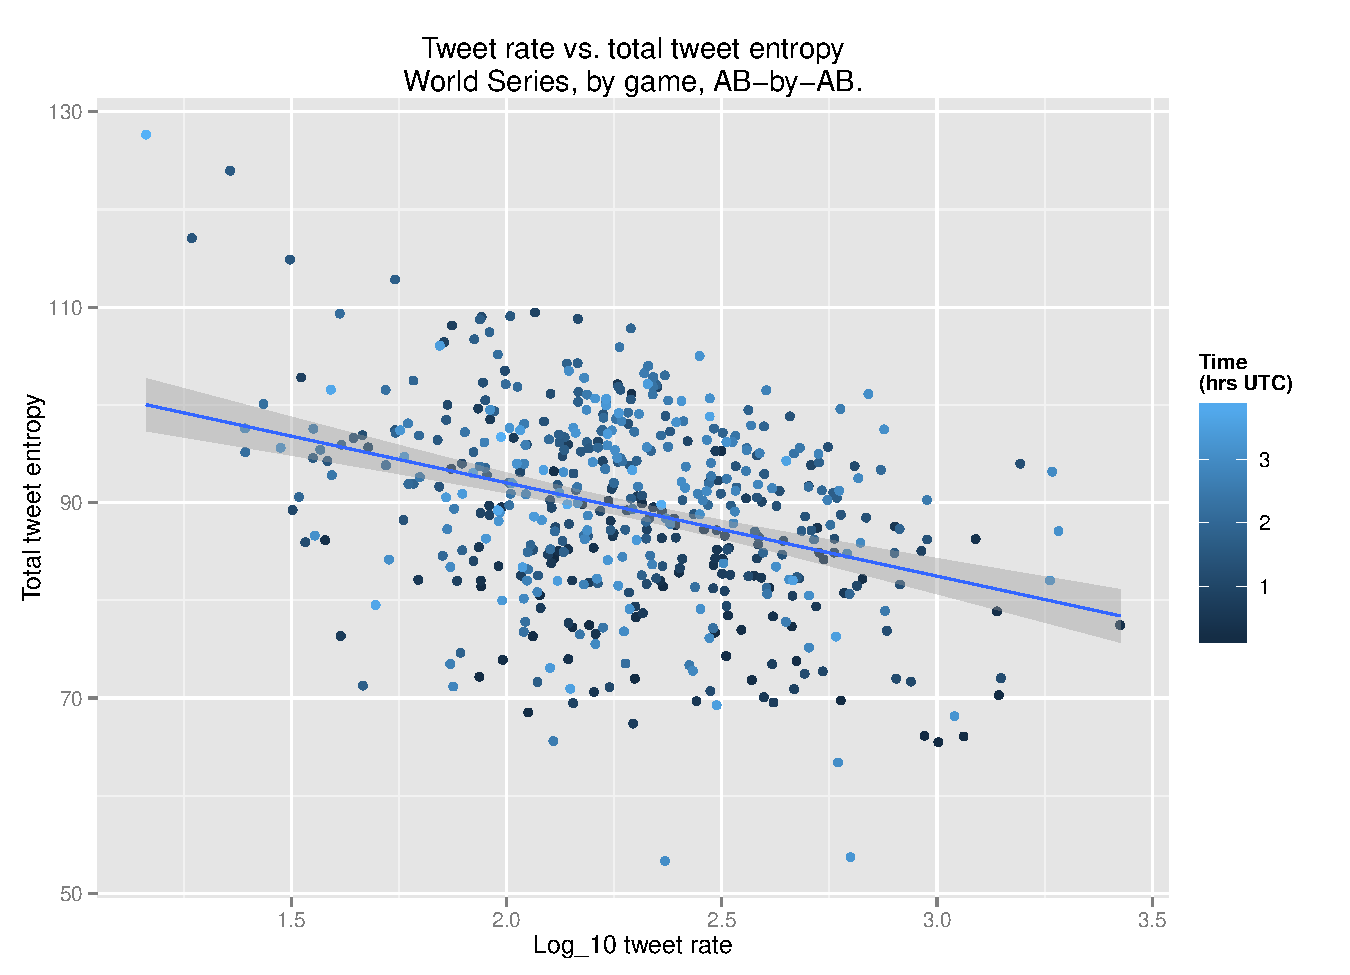
\includegraphics[width=3.25in]{figures/rate-total-ent-agg}
 \caption{Total tweet entropy plotted against log tweet rate. Color reflects in-game time; line shows the best linear fit with 95\% confidence intervals.}\label{fig:time-perword-ent}\vspace*{-.5em}
\end{figure}

\begin{table*}
  \begin{tabular}{clc}
Log rate & Tweet & Per-word entropy \\
%\hline
%2.61 & Butler channeled his inner "The Little Engine That Could" running the bases! \#Royals \#Game7 \#WorldSeries & 6.30\\
%2.61 & Was \#Butler Running Is Slo-Mo!!! \#WorldSeries \#Game7 & 8.16\\
%2.61 & Aside from chasing after a food truck, I don't think I've ever seen Billy Butler run that fast! Hang tough, \#KC! \#WorldSeries \#Royals & 7.70\\
\hline
2.49 & Fuck you, Blanco. \#Giants \#WorldSeries & 5.54\\
2.49 & Holy shitballs, @Royals! \#WorldSeries \#Game7 & 3.99\\
2.49 & Just when you thought the \#WorldSeries was over.... \#E8 & 4.76\\
\hline
1.66 & \parbox[][6ex][c]{.7\textwidth}{I suppose I appreciate Bochy's ``ASG'' approach with Bumgarner. Of course, who are any of us to question him in late October? \#WorldSeries} & 7.42\\[3pt]
1.66 & \parbox[][6ex][c]{.7\textwidth}{The guy in Marlins gear behind home plate needs to escorted off property for annoying everybody. \#WorldSeries \#WhoDoesThat} & 4.85\\[3pt]
1.66 & Lets Go Giants!!! 5-0  \#SFGiants \#WorldSeries & 3.26\\
\hline
  \end{tabular}
 \caption{Example tweets, grouped by tweet rate.}\label{tab:ex2}
\end{table*}

Our second analytic goal was to examine fast changes in information content in response to transient in-game events. Table \ref{tab:ex2} shows some examples of tweets after high-rate and low-rate events, along with their information content. Intuitively, after an exciting, game-changing event, tweets are shorter and make more reference to the shared knowledge that a particular event has just happened. The top triplet comes from one of the highest-rate at-bats, in which Gregor Blanco committed a crucial error to put the Royals in position to win the series, which these tweets all refer to.  The bottom triplet comes from a low-rate at-bat, mid-game in a developing blowout, and the tweets all have different referents as there is no salient shared event to refer to.

This short-timescale adaptation is predicted for two reasons. First, it represents a rational response to issues of information overload, the state where the amount of incoming information exceeds a user's ability to process it \cite{miller1956}.  Previous investigations into online forum posting behavior have shown such rational responses on a longer timescale \cite{jones2001a,jones2001b,whittaker2003,schoberth2003}, as well as the more explicitly conversational setting of IRC chat channels \cite{jones2008}.  Second, given that the hashtagged tweets are tied to an ongoing real-world event, changes in tweet rates are likely to be tied to what is happening in the event, providing a potential proxy for the non-linguistic context available at the time of the tweet. We will expand on this second explanation in Section \ref{sect:other-metrics}.

This trend is reflected more strongly in total entropy (and length) than in per-word entropy. STATS

\section{Control Analyses}

\subsection{Non-Rate Metrics of Context}\label{sect:other-metrics}

\subsection{Speaker Normalization}

An alternative hypothesis for the observed behavioral changes with tweet rate is that they arise not from changes in the behavior of individuals but rather from a change in demographics.  It is plausible that rising tweet rates come from an influx of new tweeters into the hashtag, and that these new tweeters simply produce shorter, less informative tweets in general.  For instance, spambots often include trending hashtags in their spam tweets \cite{martinez2013}.

To account for this, we treat the users whose tweets are in our corpus as a ``computational focus group'' \cite{lin2013,lin2014}, and collect a further 100 tweets outside the timeframe of the game for each of them.  The mean length of these tweets is the treated as a baseline for each user, and we can use the number of characters above or below the user's average tweet length to show that the adaptations to tweet rate exist at individual level.

[Plot to come, still waiting on some users.]



\section{Discussion}


\section*{Acknowledgments}

We gratefully acknowledge the support of ONR Grant N00014-13-1-0287.

\bibliographystyle{naaclhlt2015}
\bibliography{tweetprag}

\end{document}
